% Fakesection 序言之前

\RequirePackage[l2tabu, orthodox]{nag}
\RequirePackage{ifxetex}
\RequireXeTeX
\documentclass{ctexart}

%颜色
\usepackage{xcolor}

%长度
\usepackage{printlen}
\uselengthunit{mm}

%图形
\usepackage{media9}
\usepackage{pdfpages}
\usepackage{overpic}
\usepackage{graphicx}
\graphicspath{{./src/}}
\usepackage{wallpaper}
\usepackage{wrapfig}
\usepackage{pstricks}
\usepackage{smartdiagram}
\usepackage[edges]{forest}
\usepackage{pgfplots}
\usepackage{tikz}
\usetikzlibrary{shapes.geometric}
\usetikzlibrary{calc}
\usetikzlibrary{patterns}
\usetikzlibrary{arrows}
\usetikzlibrary{shapes}
\usetikzlibrary{chains}
\usetikzlibrary{mindmap}
\usetikzlibrary{graphs}
\usetikzlibrary{decorations.text}
\usetikzlibrary{arrows.meta}
\usetikzlibrary{shadows.blur}
\usetikzlibrary{shadings}
\usepackage{scsnowman}
\usepackage{tikzpeople}
\usepackage{tikzducks}
\usepackage{pifont}
\usepackage{marvosym}
\usepackage{fontawesome}
\usepackage{stmaryrd}
\usepackage{ean13isbn}
\usepackage{qrcode}
\usepackage{pgf-pie}
\usepackage{pgfmath}

%表格
\usepackage{tabu}
\usepackage{longtable}
\usepackage{booktabs}
\usepackage{diagbox}
\usepackage{multicol}
\usepackage{multirow}
\usepackage{makecell}
\usepackage{fancybox}
\usepackage{colortbl}
\usepackage{tcolorbox}
\tcbuselibrary{skins}
\tcbuselibrary{breakable}
\tcbuselibrary{theorems}
\tcbuselibrary{listings}
\tcbuselibrary{xparse}
\usepackage{fvextra}
\usepackage{csvsimple}
\usepackage{boxedminipage2e}

%公式
\usepackage{amsmath}
\usepackage{amsthm}
\usepackage{amsfonts}
\usepackage{amssymb}
\usepackage{amsbsy}
\usepackage{amsopn}
\usepackage{amstext}
\usepackage{mathrsfs}
\usepackage{bm}
\usepackage{textcomp}
\usepackage{latexsym}
\usepackage{exscale}
\usepackage{relsize}
%\usepackage{xymtex}
\usepackage{physics}
\usepackage{siunitx}
\usepackage{hologo}
\usepackage{cases}

%正文
\usepackage{fancyhdr}
\usepackage{geometry}
\usepackage{lastpage}
\usepackage{indentfirst}
\usepackage{setspace}
\renewcommand\arraystretch{1.5}

%非正文
\usepackage{makeidx}
\makeindex
\usepackage{epigraph}
\usepackage{varwidth}

%参考文献
\usepackage{morewrites}
\renewcommand{\thefootnote}{\fnsymbol{footnote}}
\usepackage[resetlabels]{multibib}
\newcites{sec}{参考网站}

%%链接
\usepackage
[	colorlinks = true,
linkcolor = gray,
citecolor = gray,
backref=page
]{hyperref}
\usepackage{caption}
\usepackage{subcaption}

%其它
\usepackage{atbegshi}
\usepackage{lipsum}

%文字
\usepackage{csquotes}
\usepackage{microtype}

\csname
endofdump
\endcsname

%\usepackage[notref,notcite]{showkeys}

%%代码
\usepackage{minted}
\tcbuselibrary{minted}% 用minted排版代码
%Java %与mcode冲突
% \usepackage{lstcustom}
%Matlab %与lstcustom冲突
%\usepackage[framed,numbered,autolinebreaks,useliterate]{mcode}
%\usepackage{boxie}
%\makeatletter
%\xdefinecolor{tcbcol@back}{rgb}{0,0,0}
%\makeatother

%枚举%与beamer冲突
\usepackage{enumitem}
\setlist[enumerate, 2]
{	fullwidth,
	label = \alph*.,
	font = \textup,
	itemindent=2em
}

\usepackage{titlesec}
%\titleformat{\chapter}{\centering\Huge\bfseries}{实验\chinese{chapter}~}{4mm}{}
\titleformat{\section}{\heiti\zihao{4}\bfseries}{\arabic{section}~}{0pt}{\vspace{12pt}}[\vspace{12pt}]
\titleformat{\subsection}{\heiti\zihao{-4}\bfseries}{\arabic{section}.\arabic{subsection}~}{0pt}{\vspace{6pt}}[\vspace{6pt}]
\titleformat{\subsubsection}{\zihao{-4}}{ (\arabic{subsubsection}) ~}{0pt}{}
\titleformat{\paragraph}{\zihao{-4}}{第\chinese{paragraph},}{0pt}{}

\begin{document}

% Fakesection 扉页

\begin{titlepage}
	\centering
	\makebox[4\ccwd][s]{}

	\vspace{40mm}
	\textbf{\fontsize{25pt}{\baselineskip}\kaishu{南京理工大学经济管理学院}}

	\vspace{5mm}
	\textbf{\fontsize{33pt}{\baselineskip}\lishu{课程论文}}

	\vspace{20mm}
	\begin{table}[htpb]
		\centering
		\songti
		\zihao{3}
		\begin{tabu}to.8\linewidth{@{}X[4,r]@{}X[c]@{}X[14,l]@{}}
			\makebox[4\ccwd][s]{课程名称}&:&\underline{\makebox[14\ccwd][c]{财务分析}}\\
			\makebox[4\ccwd][s]{论文题目}&:&\underline{\makebox[14\ccwd][c]{基于摩托摩拉的财务风险分析}}\\
			\makebox[4\ccwd][s]{姓名}&:&\underline{\makebox[14\ccwd][c]{吴振宇}}\\
			\makebox[4\ccwd][s]{学号}&:&\underline{\makebox[14\ccwd][c]{916101630117}}\\
			\makebox[4\ccwd][s]{成绩}&:&\underline{\makebox[14\ccwd][c]{}}\\
			\makebox[4\ccwd][s]{时间}&:&\underline{\makebox[14\ccwd][c]{\today}}
		\end{tabu}
	\end{table}
\end{titlepage}

% Fakesection 评分

\thispagestyle{empty}

\begin{boxedminipage}{\linewidth}
	\zihao{4}

	任课老师评语:

	\vspace{40mm}

	\begin{flushright}
		签名: \underline{\makebox[6\ccwd][c]{}}

		年\makebox[2\ccwd][c]{}月\makebox[2\ccwd][c]{}日
	\end{flushright}

	\vspace{20mm}

\end{boxedminipage}

% Fakesection 摘要

\title{\heiti\zihao{2}\textbf{基于摩托摩拉的财务风险分析}}
\author{\kaishu\zihao{4}\textbf{916101630117~吴振宇} }
\date{}
\maketitle

{
	\setlength{\baselineskip}{18pt}
	\kaishu

	\renewcommand{\abstractname}{}
	\begin{abstract}
		\zihao{5}
		\noindent
		\textbf{摘要:} 经济全球化下,市场经济发展逐渐完善,通过战略投资以获取更多收益已经成为企业快速扩张的重要途径之一。但投资存在的风险与收益的正比性也往往使许多企业一步失误而全盘皆输。本文以摩托罗拉公司的失败案例作为分析对象,得到结论:作为企业的管理层,应当牢牢将财务风险的管理贯穿生产运营的全过程,制定战略前经过充分调查,执行战略期间时刻把控形势,以达到趋利避害,将可控风险降到最低。
	\end{abstract}

	\textbf{关键词:}战略投资;财务风险;可控风险;摩托罗拉。

	\renewcommand{\abstractname}{}
	\begin{abstract}
		\zihao{5}
		\noindent
		\textbf{Abstract: }Under the economic globalization, the development of market economy is gradually improving. It has become one of the important ways for enterprises to expand rapidly to obtain more profits through strategic investment. However, the proportionality of risks and returns in investment often causes many enterprises to fail one step and lose the whole game. This paper takes the failure case of Motorola Company as the object of analysis and draws the conclusion that as the management of enterprises, financial risk management should be firmly throughout the whole process of production and operation, fully investigated before formulating the strategy, and control the situation at all times during the implementation of the strategy, in order to achieve the goal of seeking benefits and avoiding disadvantages, and to minimize the controllable risk.
	\end{abstract}

	\textbf{Key Words: }Strategic investment; Financial risk; Controllable risk; Motorola.

}

%页眉页脚%与book冲突
\pagestyle{fancy}
%\renewcommand{\headrulewidth}{0pt}
\lfoot{\small{\leftmark}}
\cfoot{\small{第\thepage 页~共~\pageref{LastPage}~页}}
\rfoot{\small{\rightmark}}

\setcounter{page}{1}

\section{引言}%
\label{sec:引言}

在当今全球化的浪潮之下,企业如果固守自己已有的收益,不再求图进取,将会过早地进入企业的衰败期。如何持续保持企业的发展能力,稳定在企业的成熟期是众多已经有一定发展基础的大型、中型企业正面临的难题。而通过合理的战略投资,开拓新的市场、获取新的收益则是一项合适的策略。

但风险与收益往往是成正比的,为了获取看似客观的收益而铤而走险,从而导致企业由盛转衰,从而过早的进入衰败期的案例数不胜数。

因此,对企业的财务风险,特别是因战略投资错误而导致的财务分析进行分析,不仅具有理论上的价值,也具有一定的现实意义。\cite{孙瑞娟2010企业并购财务风险的分析与防范}

\begin{figure}[htpb]
	\centering
	\tikzset{
		planet/.append style={regular polygon, regular polygon sides=6},
		satellite/.append style={regular polygon, regular polygon sides=6},
		every picture/.append style={rotate=30},
		connection planet satellite/.style={
			bend right/.style=,
			every edge/.style={fill=\col},
			to path={
				\pgfextra
				\path[draw=none, fill=none] (\tikztostart)
				-- coordinate[at start] (@start@) coordinate[at end] (@target@) (\tikztotarget);
				\endpgfextra
				\ifnum\xi<\maxsmitem % to disable the last arrow
					($(@start@)!.6cm!90:(@target@)$) -- ($(@target@)!.25cm!-90:(@start@)$)
					-- ($(@target@)!.25cm!90:(@start@)$) -- ($(@start@)!.6cm!-90:(@target@)$)
					-- cycle
	\fi}}}
	\smartdiagram[connected constellation diagram]{
		企业\\生命\\周期,
		设立,
		发展,
		成长,
		成熟,
		衰退,
		倒闭
	}
	\caption{企业生命周期}
	\label{fig:企业生命周期}
\end{figure}

\subsection{财务风险}%
\label{sub:}

企业财务风险是指在各项财务活动过程中,由于各种难以预料或控制的因素影响,财务状况具有不确定性,从而使企业有蒙受损失的可能性。按财务活动的主要环节,可以分为流动性风险、信用风险、筹资风险、投资风险。按可控程度分类,可分为可控风险和不可控风险。按产生原因,可分为战略风险、运营风险、内部监控失效、金融风险、法律风险。

\begin{figure}[htpb]
	\centering
	\forestset{
		direction switch/.style={
			for tree={edge+=thick, font=\sffamily},
			where level>=1{folder, grow'=0}{for children=forked edge},
			where level=3{}{draw},
		},
	}
	\begin{forest}
		% forest preamble: determine layout and format of tree
		direction switch
		[财务风险
		[财务活动主要环节
		[流动性风险]
		[信用风险]
		[筹资风险]
		[投资风险]
		]
		[可控程度
		[可控风险]
		[不可控风险]
		]
		[产生原因
		[战略风险]
		[运营风险]
		[内部监控失效]
		[金融风险]
		[法律风险]
		]
		]
	\end{forest}
	\caption{财务风险分类}
	\label{fig:财务风险分类}
\end{figure}

财务风险客观存在,企业不可能消除财务风险,只能采取措施将财务风险对企业的危害降到最低。充分认识财务风险形成的原因,是采取有效措施的前提。本文将针对产生原因中的战略投资错误进行具体分析,并给出相关结论。

\section{案例简介}%
\label{sec:案例简介}

摩托罗拉 \footnote{(Motorola Inc )} ,是一家总部设在美国伊利诺伊州绍姆堡,位于芝加哥市郊。世界财富百强企业之一,是全球芯片制造、电子通讯的领导者。主要经营业务有消费电子、移动通信、互联网等,产品有通讯产品、网络产品、软件等。

\begin{figure}[htpb]
	\centering
	
\includegraphics[width=0.5\linewidth]{motorola.jpg}
	\caption{摩托罗拉徽标}
	\label{fig:摩托罗拉徽标}
\end{figure}

10 年前,摩托罗拉还一直是引领尖端技术和卓越典范的代表,享有着全球最受尊敬公司之一的尊崇地位。它一度前无古人地每隔 10 年便开创一个工业领域,有的 10 年还开创两个。成立 80 年来,发明过车载收音机、彩电显像管、全晶体管彩色电视机、半导体微处理器、对讲机、寻呼机、大哥大 (蜂窝电话 )以及“六西格玛”质量管理体系认证,它先后开创了汽车电子、晶体管彩电、集群通信、半导体、移动通信、手机等多个产业, 并长时间在各个领域中找不到对手。

在1995年摩托罗拉在中国的市场占有率高达60\%以上,而仅仅过去了10年,就已经跌至12\%不到。思考其原由不由令人唏嘘。\cite{吴定祥2015中国联想并购摩托罗拉案例分析}

\section{财务风险}%
\label{sec:财务风险}

这样一家有着煊赫历史的企业,在 2003 年手机的品牌竞争力排在第一位, 2004 年被诺基亚超过排在了第二位,而到了 2005 年,则又被三星超过,排到了第三位。早在 2008 年 5 月,市场调研厂商 IDC 和战略分析公司Strategy Analytics 表示,摩托罗拉可能在 2008 年底之前失去北美市场占有率第一的位置。摩托罗拉的当季报也显示,2008 年第一季度全球手机销量下降 39\%, 手机部门亏损 4.18亿美元,与上年同期相比亏损额增加了 80\%。

\begin{figure}[htpb]
	\centering
	\begin{tikzpicture}
		\begin{axis}[ybar,enlargelimits=0.15]  % 绘制关于y坐标的条形图,条形之间的最大间隔是0.15cm
			\addplot[draw=blue,fill=red]           % 蓝色边界、红色填充
				coordinates
				{
					(1,99.93) (2,94.09) (3,89.63) (4,88.81)
				};
			\addplot[draw=black,fill=blue]         % 黑色边界、蓝色填充
				coordinates
				{
					(1,110.83) (2, 106.85) (3, 103.58) (4, 103.73)
				};
			\addlegendentry{资产/负债 (亿) };
		\end{axis}
	\end{tikzpicture}
	\caption{2018年各季度资产/负债}
	\label{fig:2018年各季度资产/负债}
\end{figure}

\newpage

\begin{table}[htpb]
	\centering
	\caption{资产负债表}
	\label{tab:资产负债表}
\end{table}
\csvautobooklongtable{src/motorola.csv}

根据资产负债表,可见负债的规模正在逐年增长,负债方面存在着比较大的上升\%。企业负债规模会影响企业的发展,显而易见,企业负债规模过大,就会产生企业利息支出增大的问题,企业的收益也会相应的减少,偿付能力就会减弱,使得筹资风险增大。在企业的总负债当中,由于长期和短期负债占比不可能完全相同,缺乏合理安排长期负债的比例,增加了企业融资的风险。资产规模也在逐年增长,企业偿还债务的能力逐年减弱,存在一定的财务风险。

\section{发展战略}%
\label{sec:发展战略}

为了夺得对世界移动通信市场的主动权,并实现在世界任何地方使用无线手机通信,以摩托罗拉为首的美国一些公司在政府的帮助下,于 1987 年提出新一代卫星移动通信星座系统——铱星。

铱星系统技术上的先进性在目前的卫星通信系统中处于领先地位。铱星系统卫星之间可通过星际链路直接传送信息,这使得铱星系统用户可以不依赖地面网而直接通信,但这也恰恰造成了系统风险大、成本过高、维护成本相对于地面也高出许多。整个卫星系统的维护费一年就需几亿美元之巨。

\begin{figure}[htpb]
	\centering
	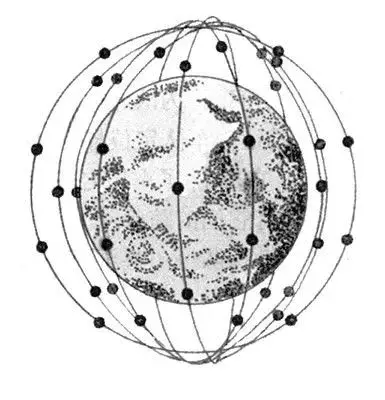
\includegraphics[width=0.5\linewidth]{77.png}
	\caption{铱星计划}
	\label{fig:铱星计划}
\end{figure}

铱星的高科技含量举世公认,但铱星手机价格每部高达 3000 美元,加上高昂的通话费用,它开业的前两个季度,在全球只发展了 1 万用户,这使得铱星公司前两个季度的亏损即达 10 亿美元。尽管铱星手机后来降低了收费,但仍未能扭转颓势。

\section{营销战略}%
\label{sec:营销战略}

\subsubsection{产品开发方向不够明确}%
\label{ssub:产品开发方向不够明确}


不考虑手机的细分发展, 3年时间仅依赖 V3 一个机型。没有人会否认 V3 作为一款经典手机的地位,正是依靠 V3,摩托罗拉 2005 年全年利润提高了 102\%,手机发货量增长 40\%,摩托罗拉品牌也重焕生机。尽管 V3 让摩托罗拉重新复苏,更让摩托罗拉看到了夺回市场老大的希望。然而,摩托罗拉过分陶醉于 V3 带来的市场成功。赛迪顾问研究显示, 2005 年以前是明星机型的天下,一款明星手机平均可以畅销 2-3 年,而过了 2005 年,手机市场已成了细分市场的天下,手机行业已经朝着智能化、专业拍照、娱乐等方向极度细分, 而摩托罗拉似乎对此视而不见。在中国市场, 2007 年摩托罗拉仅仅推出 13 款新机型,而其竞争对手三星推出了 54 款机型,诺基亚也有 37 款。——价格跳水快,自毁品牌形象。在新品跟不上的情况下,降价成了摩托罗拉提高销量不得不采取的手段。许多摩托罗拉的忠实用户把摩托罗拉的手机称为“ (价格 )跳水冠军” 。以 V3 为例,从刚上市时的 6000 多元的高端时尚机型跌入 4000 多元的白领消费群,再到 2000 多元的普通时尚消费群,直到停产前的 1200 多元。短期的大幅降价让不少高端用户无法接受,同时也对 V3 的定位产生了质疑,后果就是对摩托罗拉品牌彻底失去信任。

\subsubsection{产品与市场需求脱轨}%
\label{ssub:产品与市场需求脱轨}

手机消费者在手机厂商的培育和自发发展下,需求变化日益飘忽不定。消费者对手机的要求已经不仅仅局限在外观方面,苛刻的消费者更多地开始关注手机的配置、功能特色等内在技术因素。以技术见长的摩托罗拉本不应在技术方面让消费者失望,但是现实还是让消费者失望了。从手机零售卖场那些列出来的一目了然的参数中,摩托罗拉的像素、屏幕分辨率、内存几乎都落后于诺基亚等竞争对手的同类机型。自从推出 V3 之后,摩托罗拉发布的绝大部分新品手机无论是 U 系还是 L 系, 甚至是K 系就再也抹不去 V3 的影子,尤其是其金属激光蚀刻键盘设计。 V3 的键盘设计的确是经典,但再经典的东西被反反复复无数次拿出来用,也会引起消费者的视觉疲劳,甚至产生抵触情绪,尤其是对于那些换机用户。

\section{运营战略}%
\label{sec:运营战略}

摩托罗拉是一个很重视产品规划的公司,此前摩托罗拉每开发一款新产品,通常先提前数月预测消费趋势。但在快速升级换代的手机行业中,制造商们试图提前数月预测消费者需求是非常困难的。

再加上摩托罗拉是一家技术主导型的公司,工程师文化非常浓厚,这种公司通常以自我为中心,唯“技术论” ,从而导致摩托罗拉虽然有市场部门专门负责收集消费者需求的信息,但在技术导向型的企业文化里,消费者的需求很难被研发部门真正倾听,研发部门更愿意花费大量精力在那些复杂系统的开发上,从而导致研发与市场需求的脱节。

另外,摩托罗拉内部产品规划战略上的不统一、 不稳定,还使得上游的元器件采购成本一直降不下来,摩托罗拉每一个型号都有一个全新的平台,平台之间大多不通用,这就带来生产、采购、规划上的难度。对于全球顶级通信设备商而言,同时运营好系统设备和手机终端两块业务,似乎是一项“不可能完成的任务” 。

\section{总结}%
\label{sec:总结}

根据分析结果,可以得到以下结论:

\begin{description}
	\item[提高财务决策的科学水平]只有提高财务决策的科学水平,才能防止因决策失误而产生的财务风险。正如摩托罗拉公司的发展战略、营销战略制定的严重失误,为之后的财务风险埋下了隐患。企业必须采用科学的决策方法。在决策过程中,应充分考虑影响决策的各种因素,尽量采用定量计算及分析方法,并运用科学的决策模型进行决策,对各种可行方案决策,切忌主观臆断。\cite{孙新宇2016企业财务风险识别与防范案例分析}
	\item[加强管理人员对风险的客观认识]管理者的风险意识也是财务风险相关的一个重要因素。正如摩托罗拉公司的财务危机早有征兆,而管理层却置之不理,最终招来无法挽回的后果。加强风险教育,加强业务培训,提高管理人员素质,提高风险的甄别能力。只有在对财务风险有了一定认识, 在制定决策时考虑到财务风险, 定期对企业各类财务信息加以对比分析, 找出企业潜在的风险因素,才能最大程度避免风险。
	\item[建立完善的财务管理和风险控制体系]摩托罗拉公司最终的衰败与其管理上的混乱是分不开的。财务风险的影响是可以通过财务体系的优化而尽量减小。所以,企业在确定财务风险控制目标时不能一味追求低风险甚至零风险, 而应本着成本效益原则把财务风险控制在一个合理的、可接受的范围之内。因此,要加强企业财务风险防范,如何防范企业财务风险,化解财务风险,以实现财务管理目标。\cite{赵军2011浅谈财务风险分析与防范}
\end{description}

% Fakesection 参考文献

\bibliographystyle{IEEEtran}
\bibliography{src/main}

\end{document}

